
%%%%%%%%%%%%%%%%%%%%%%%%%%%%%%%%%%%%%%%%%%%%%%%%%%%%%%%%%%%%%%%%%%%%%
%% This is a (brief) model paper using the achemso class
%% The document class accepts keyval options, which should include
%% the target journal and optionally the manuscript type.
%%%%%%%%%%%%%%%%%%%%%%%%%%%%%%%%%%%%%%%%%%%%%%%%%%%%%%%%%%%%%%%%%%%%%
\documentclass[journal=jacsat,manuscript=article]{achemso}

%%%%%%%%%%%%%%%%%%%%%%%%%%%%%%%%%%%%%%%%%%%%%%%%%%%%%%%%%%%%%%%%%%%%%
%% Place any additional packages needed here.  Only include packages
%% which are essential, to avoid problems later. Do NOT use any
%% packages which require e-TeX (for example etoolbox): the e-TeX
%% extensions are not currently available on the ACS conversion
%% servers.
%%%%%%%%%%%%%%%%%%%%%%%%%%%%%%%%%%%%%%%%%%%%%%%%%%%%%%%%%%%%%%%%%%%%%
\usepackage[version=3]{mhchem} % Formula subscripts using \ce{}

%%%%%%%%%%%%%%%%%%%%%%%%%%%%%%%%%%%%%%%%%%%%%%%%%%%%%%%%%%%%%%%%%%%%%
%% If issues arise when submitting your manuscript, you may want to
%% un-comment the next line.  This provides information on the
%% version of every file you have used.
%%%%%%%%%%%%%%%%%%%%%%%%%%%%%%%%%%%%%%%%%%%%%%%%%%%%%%%%%%%%%%%%%%%%%
%%\listfiles

%%%%%%%%%%%%%%%%%%%%%%%%%%%%%%%%%%%%%%%%%%%%%%%%%%%%%%%%%%%%%%%%%%%%%
%% Place any additional macros here.  Please use \newcommand* where
%% possible, and avoid layout-changing macros (which are not used
%% when typesetting).
%%%%%%%%%%%%%%%%%%%%%%%%%%%%%%%%%%%%%%%%%%%%%%%%%%%%%%%%%%%%%%%%%%%%%
\newcommand*\mycommand[1]{\texttt{\emph{#1}}}

%%%%%%%%%%%%%%%%%%%%%%%%%%%%%%%%%%%%%%%%%%%%%%%%%%%%%%%%%%%%%%%%%%%%%
%% Meta-data block
%% ---------------
%% Each author should be given as a separate \author command.
%%
%% Corresponding authors should have an e-mail given after the author
%% name as an \email command. Phone and fax numbers can be given
%% using \phone and \fax, respectively; this information is optional.
%%
%% The affiliation of authors is given after the authors; each
%% \affiliation command applies to all preceding authors not already
%% assigned an affiliation.
%%
%% The affiliation takes an option argument for the short name.  This
%% will typically be something like "University of Somewhere".
%%
%% The \altaffiliation macro should be used for new address, etc.
%% On the other hand, \alsoaffiliation is used on a per author basis
%% when authors are associated with multiple institutions.
%%%%%%%%%%%%%%%%%%%%%%%%%%%%%%%%%%%%%%%%%%%%%%%%%%%%%%%%%%%%%%%%%%%%%
\author{Ruchi Lohia}
%\altaffiliation{A shared footnote}
\author{Reza Salari}
%\altaffiliation{Current address: Some other place, Othert\"own,
%Germany}
\author{Grace Brannigan}
\email{grace.brannigan@rutgers.edu(GB)}
\affiliation[Rutgers University]
{Center for Computational and Integrative Biology, Rutgers University, Camden, NJ, USA}
\alsoaffiliation[Rutgers University]
{ Department of Physics, Rutgers University, Camden, NJ, USA}

%%%%%%%%%%%%%%%%%%%%%%%%%%%%%%%%%%%%%%%%%%%%%%%%%%%%%%%%%%%%%%%%%%%%%
%% The document title should be given as usual. Some journals require
%% a running title from the author: this should be supplied as an
%% optional argument to \title.
%%%%%%%%%%%%%%%%%%%%%%%%%%%%%%%%%%%%%%%%%%%%%%%%%%%%%%%%%%%%%%%%%%%%%
\title[An \textsf{achemso} demo]
  {Mechanism underlying conformational effects of the disease-associated Val66Met substitution on the intrinsically disordered region of proBDNF\footnote{A footnote for the title}}

%%%%%%%%%%%%%%%%%%%%%%%%%%%%%%%%%%%%%%%%%%%%%%%%%%%%%%%%%%%%%%%%%%%%%
%% Some journals require a list of abbreviations or keywords to be
%% supplied. These should be set up here, and will be printed after
%% the title and author information, if needed.
%%%%%%%%%%%%%%%%%%%%%%%%%%%%%%%%%%%%%%%%%%%%%%%%%%%%%%%%%%%%%%%%%%%%%
\abbreviations{IR,NMR,UV}
\keywords{American Chemical Society, \LaTeX}
% Please keep the abstract below 300 words


% Please keep the Author Summary between 150 and 200 words
% Use first person. PLOS ONE authors please skip this step. 
% Author Summary not valid for PLOS ONE submissions.   





% Use "Eq" instead of "Equation" for equation citations.


% Results and Discussion can be combined.
\begin{document}


\renewcommand{\thepage}{S\arabic{page}}  
\renewcommand{\thesection}{S\arabic{section}}   
\renewcommand{\thetable}{S\arabic{table}}   
\renewcommand{\figurename}{}
\renewcommand{\thefigure}{Fig S\arabic{figure}}

\subsubsection*{Selection of force field}
In order to get accurate structural characterization of proBDNF with MD,  we ran  500ns of T-REMD simulations of 30 residue fragment of V66 proBDNF with several commonly used ff and water model combinations. First 200ns of data was discarded as equilibration ~\ref{S1}a compares the CA shifts for  Amber99sb*-ildn-q ~\cite {Lindorff-Larsen2010a, Hornak2006a} with Tip4p-D ~\cite {Piana2015},  Amber99sbws ~\cite {Lindorff-Larsen2010a, Best2014} Amberff03sbws  ~\cite {Best2009, Best2014}, Amber99sb-ildn with Tip3P ~\cite {Jorgensen1981} and NMR.  Amber99sb-ildn with Tip4p-D and Amber99sbws gives good agreement with NMR CA chemical shift.  We also compared Rg distribution for the tested ff (~\ref{S1}b).  Tip3P generates very collapsed ensembles and the remaining three ff generates similar Rg distribution. Tip3P is known to produce structures which are too collapsed relative to experiment. ~\cite {Piana2015, Best2014, Mercadante2015} Since, the remaining three ff gives comparable Rg, we proceed with Amber99sb*-ildn-q with Tip4p-D because it gives the best match with experiments. It has also been observed that for IDP's with little or no secondary structure,  Amber99sb*-ildn-q with Tip4p-D showed good agreement with experimental NMR measurements. ~\cite {Robustelli2018}.

 \begin{figure}[!ht]
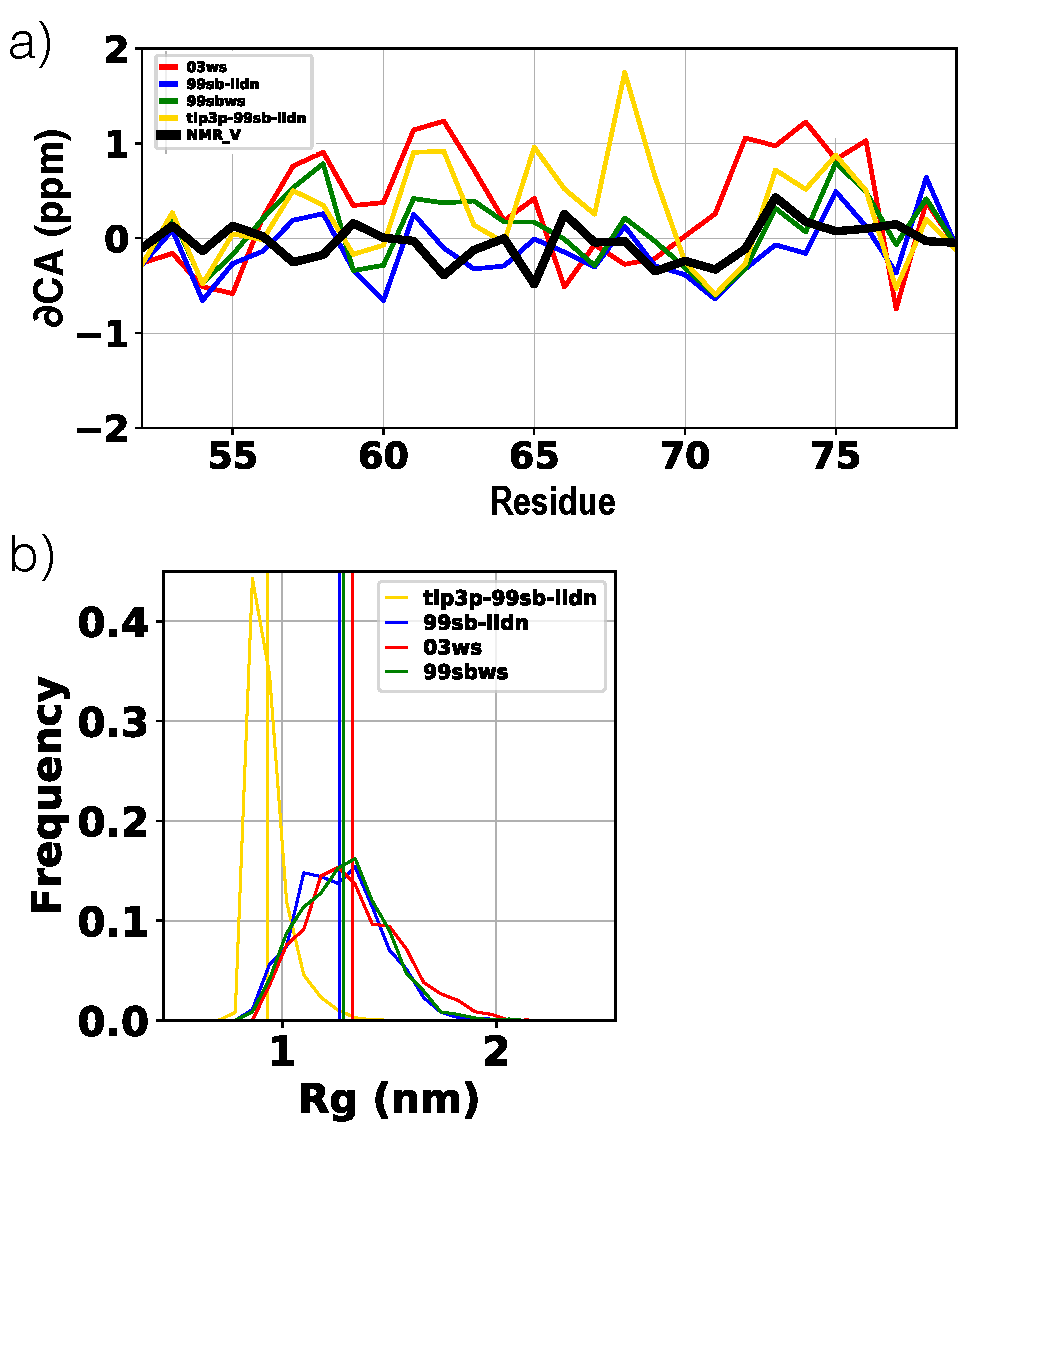
\includegraphics[scale=0.5,width=\textwidth,trim={0 0cm 0 0cm},clip]{../figures/S1.pdf}
\caption{{\bf Ff comparison.} (a) Comparison of calculated chemical shifts from MD ensembles at 280K and NMR chemical shifts from ~\cite{Anastasia2013}  at 280K,  as described in methods. (b) Rg distribution for each ff.}
\label{S1} 
\end{figure}


\subsubsection*{Comparison with NMR}

\begin{figure}[!ht]
 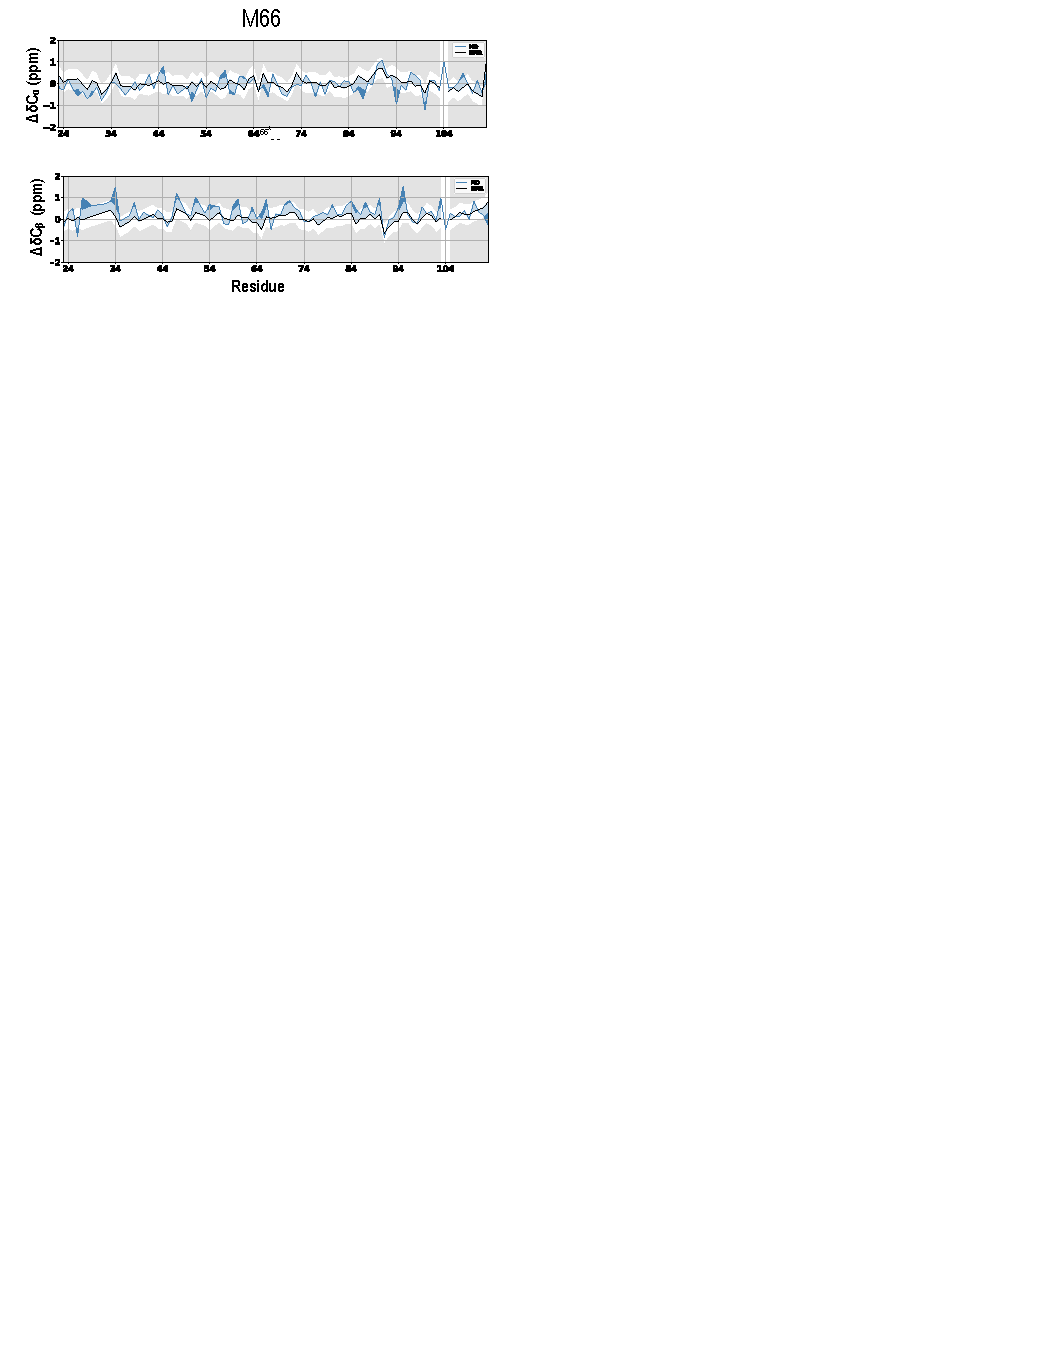
\includegraphics[scale=0.5,width=\textwidth,trim={0 0cm 0 0},clip]{../figures/S2.pdf}
\caption{{\bf Comparison of CB chemical shifts with NMR.}
.
 }
\label{S2} 
\end{figure}


\begin{figure}[!ht]
 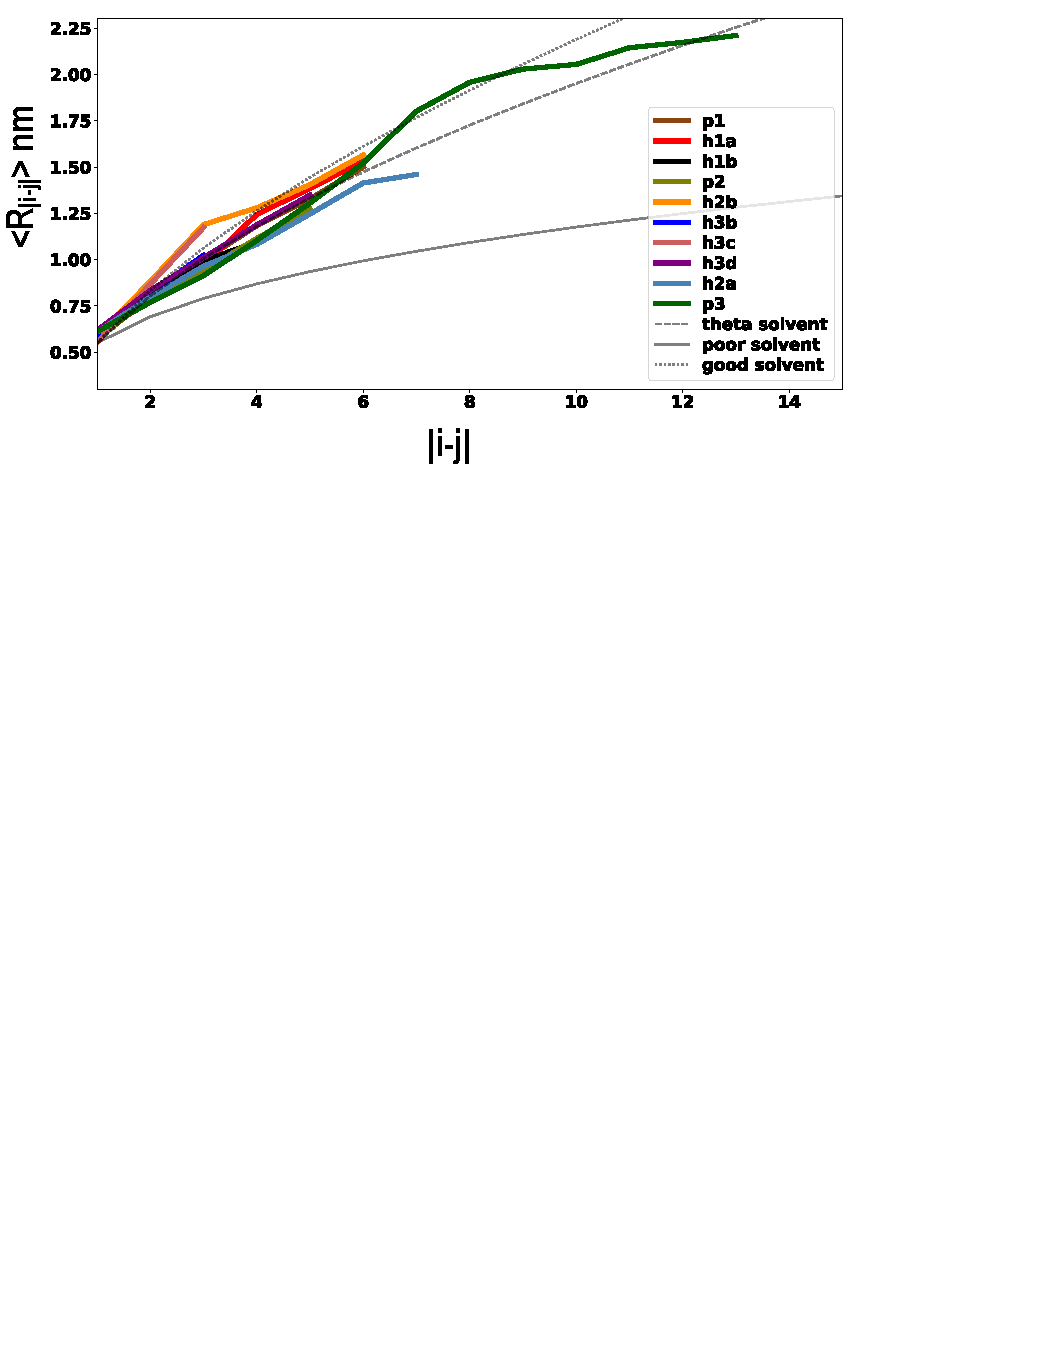
\includegraphics[scale=0.5,width=\textwidth,trim={0 0cm 0 0},clip]{../figures/S3.pdf}
\caption{{\bf Comparison of secondary structure with NMR for His65 protonated states.}
.
 }
\label{S3} 
\end{figure}

\begin{figure}[!ht]
 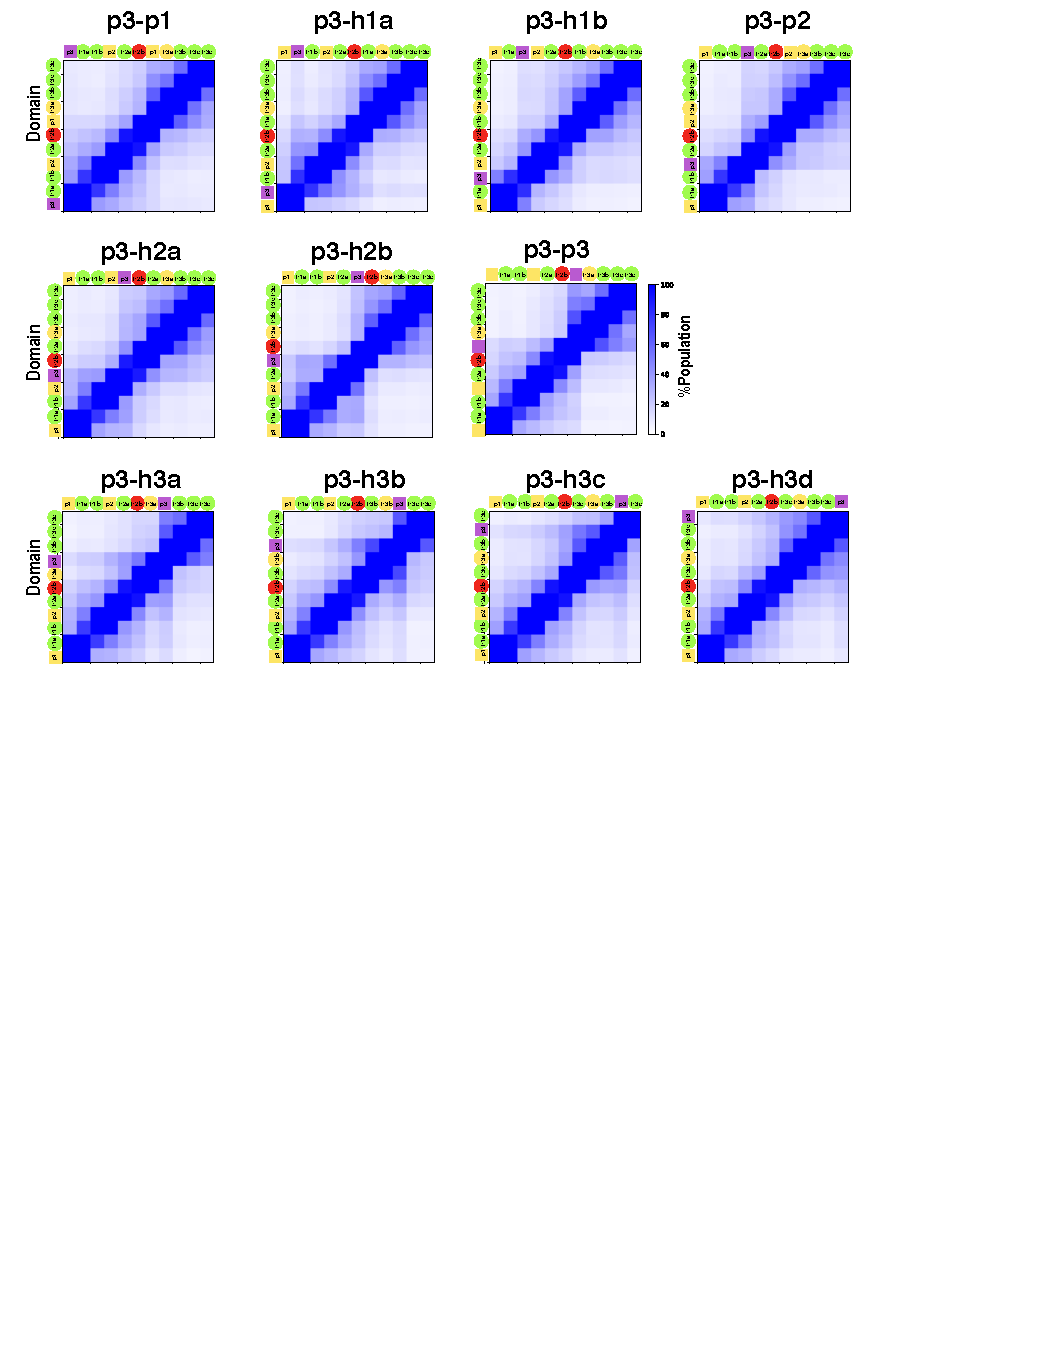
\includegraphics[scale=0.5,width=\textwidth,trim={0 0cm 0 0},clip]{../figures/S4.pdf}
\caption{{\bf Contact probablity of 2b:3b contact for V66 and M66 .}
.
 }
\label{S4} 
\end{figure}

\begin{figure}[!ht]
 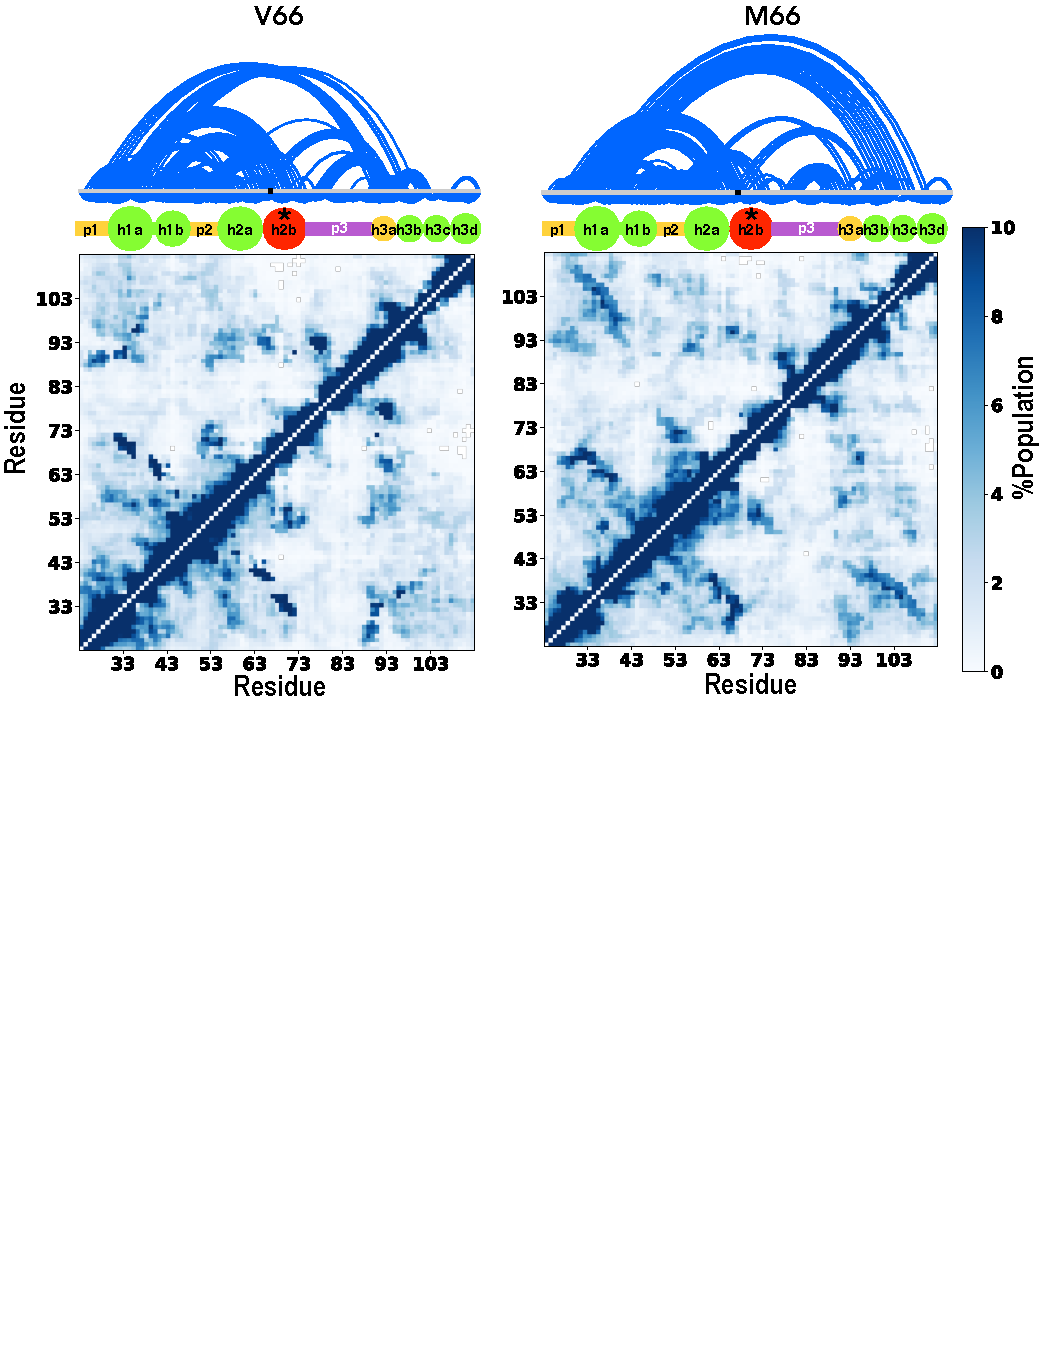
\includegraphics[scale=0.5,width=\textwidth,trim={0 0cm 0 0},clip]{../figures/S5.pdf}
\caption{{\bf Contact probability for protonated states .}
.
 }
\label{S5} 
\end{figure}

\begin{figure}[!ht]
 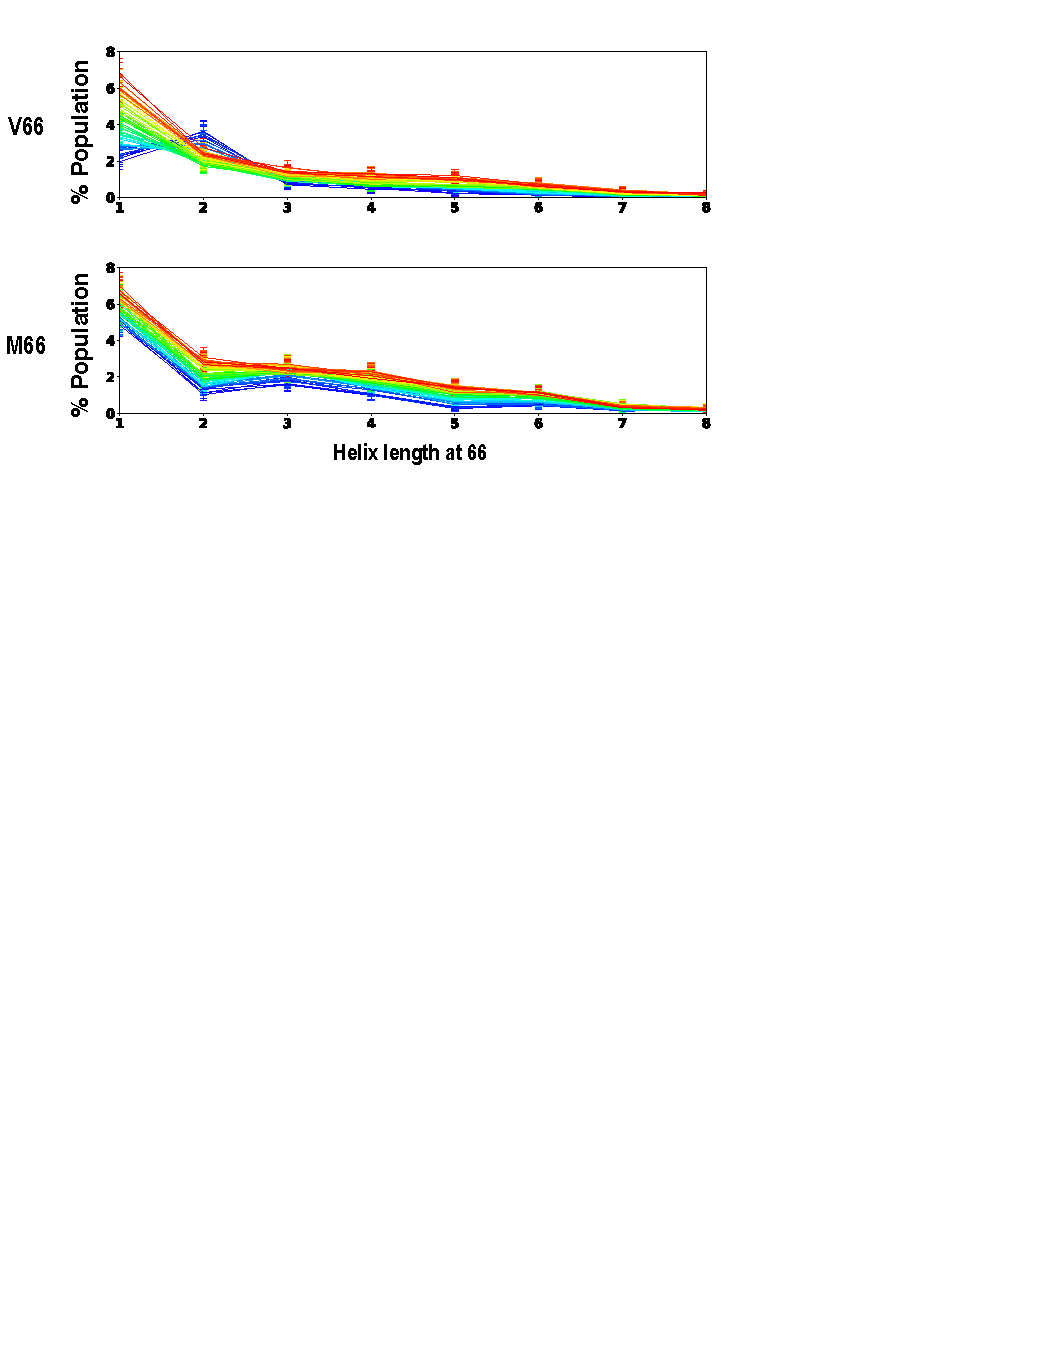
\includegraphics[scale=0.5,width=\textwidth,trim={0 0cm 0 0},clip]{../figures/S6.pdf}
\caption{{\bf Comparison of contact probability for protonated vs non-protonated states .}
.
 }
\label{S6} 
\end{figure}

\begin{figure}[!ht]
 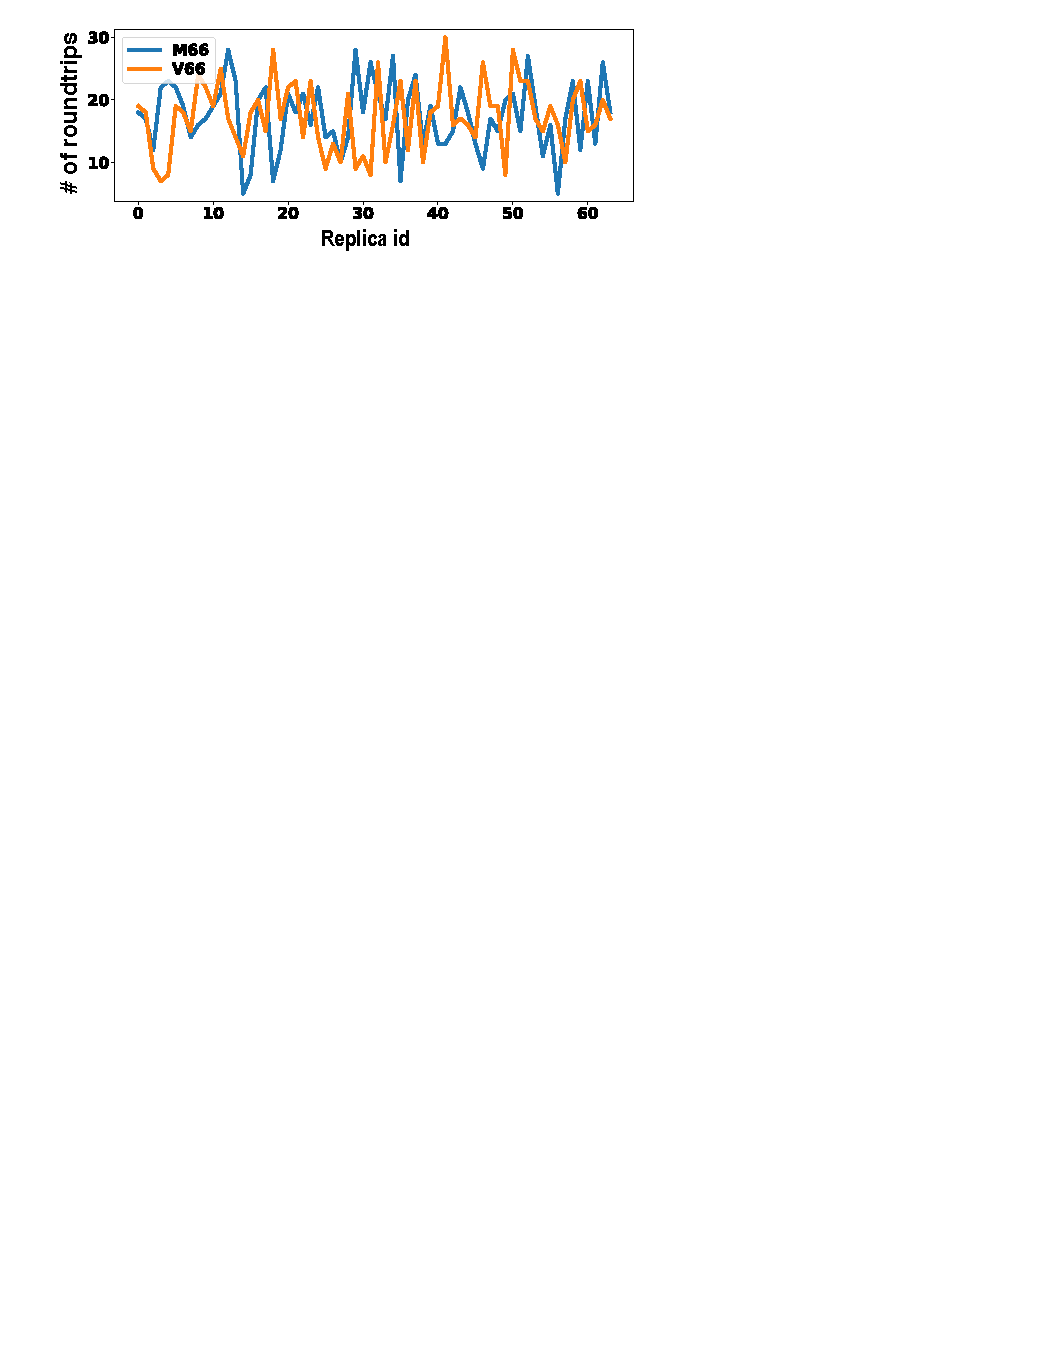
\includegraphics[scale=0.5,width=\textwidth,trim={0 0cm 0 0},clip]{../figures/S7.pdf}
\caption{{\bf Rg distribution for all four simualtions.}
.
 }
\label{S7} 
\end{figure}

\begin{figure}[!ht]
 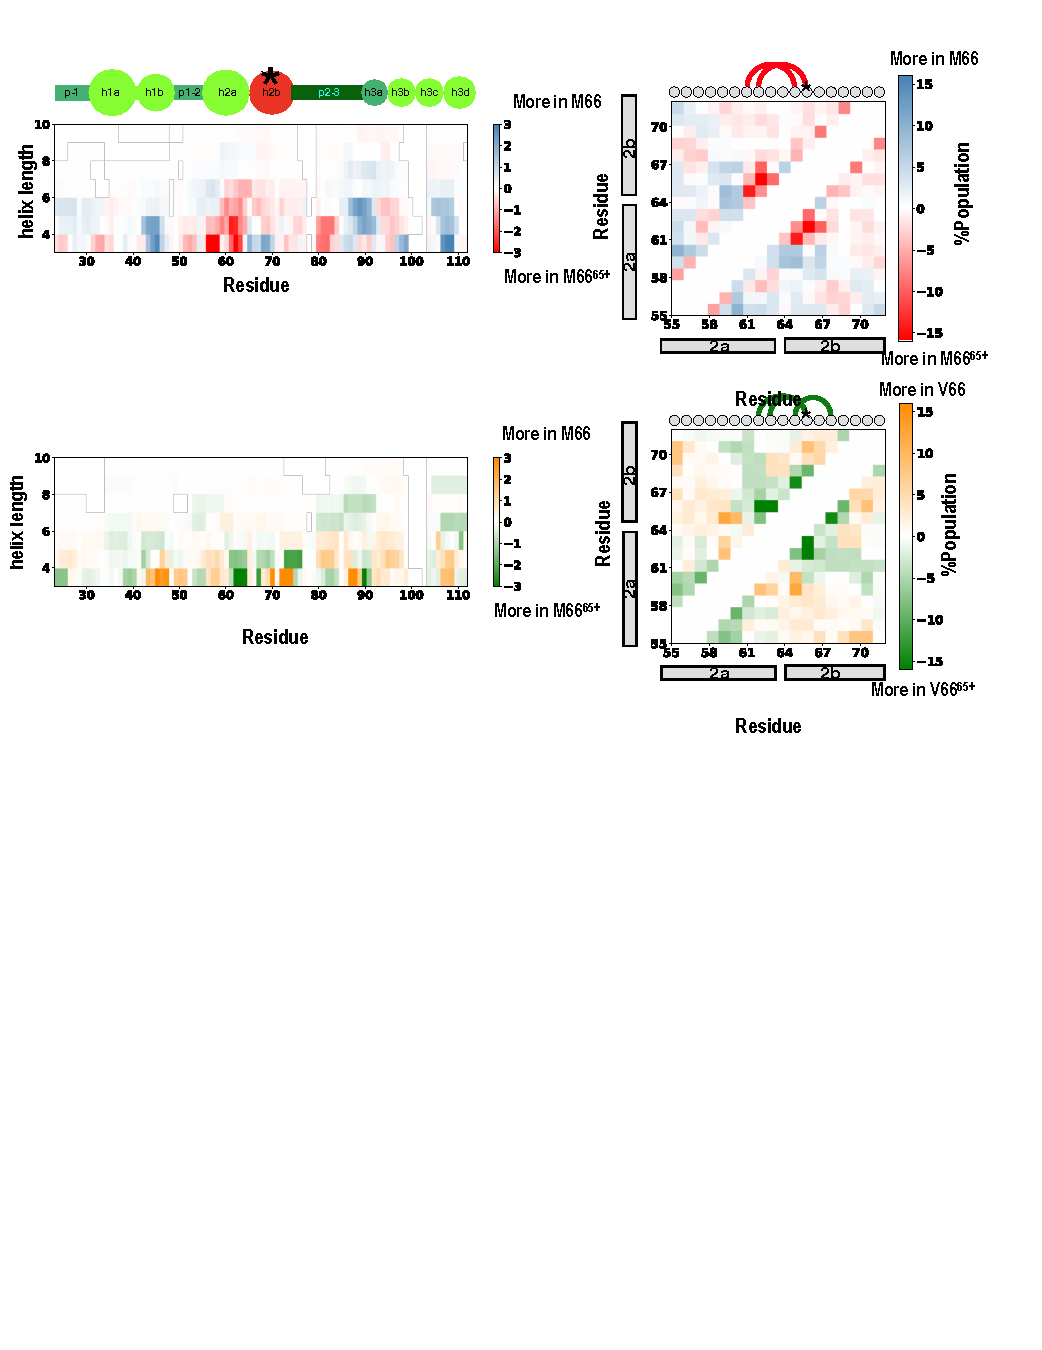
\includegraphics[scale=0.5,width=\textwidth,trim={0 0cm 0 0},clip]{../figures/S8.pdf}
\caption{{\bf Helix length and intra-domain contacts.}
.
 }
\label{S8} 
\end{figure}

\begin{figure}[!ht]
 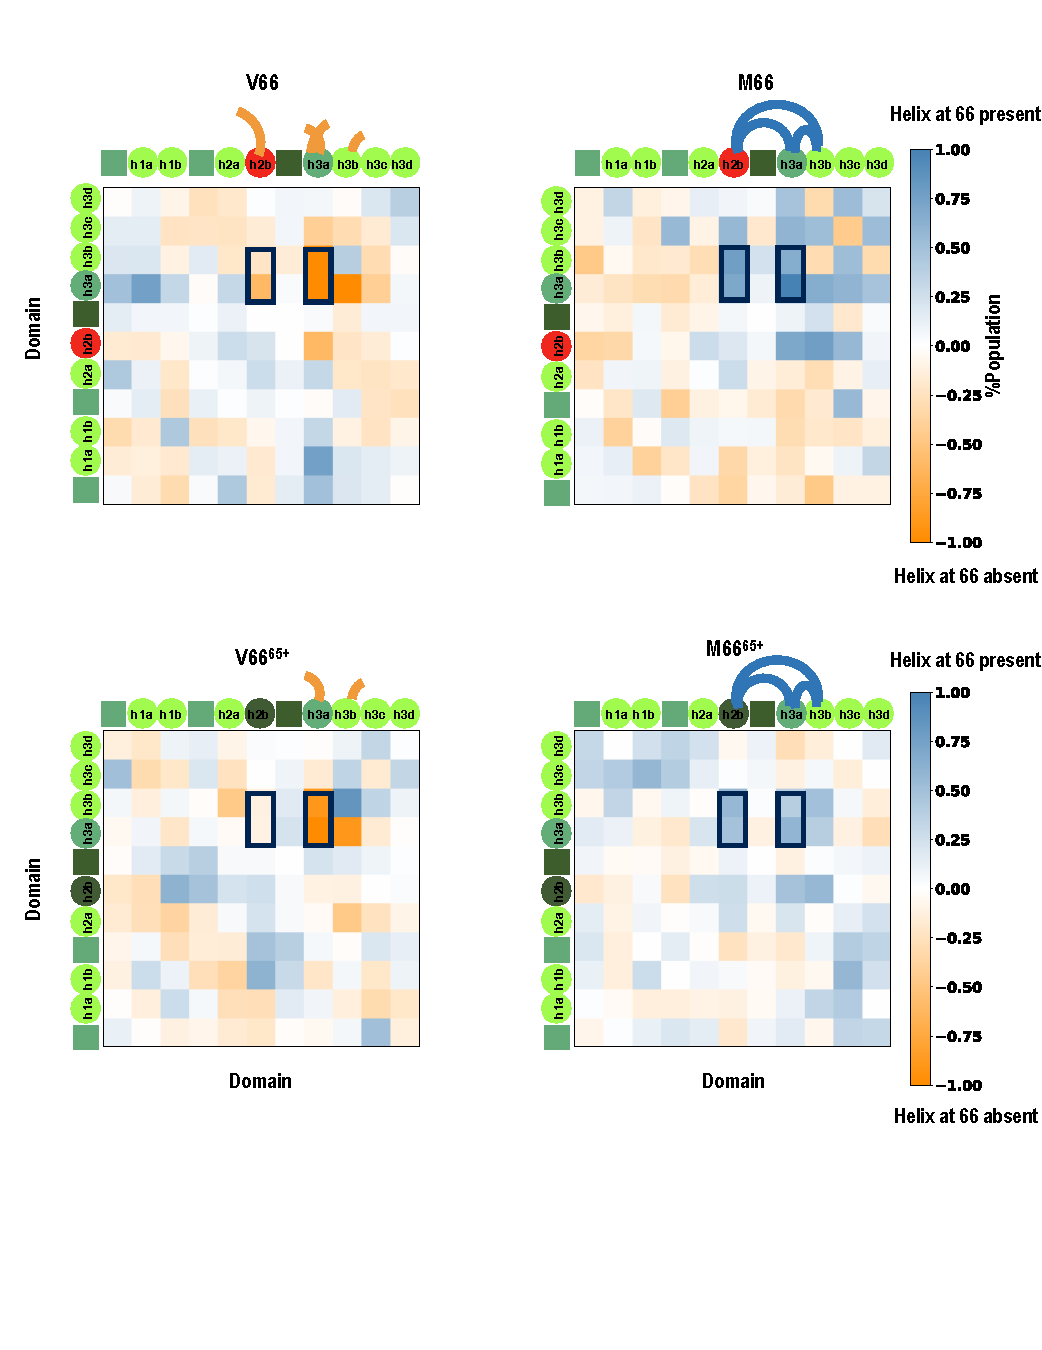
\includegraphics[scale=0.5,width=\textwidth,trim={0 0cm 0 0},clip]{../figures/S9.pdf}
\caption{{\bf Inter-domain coupling for when 66 is in helix.}
.
 }
\label{S9} 
\end{figure}
\begin{figure}[!ht]
 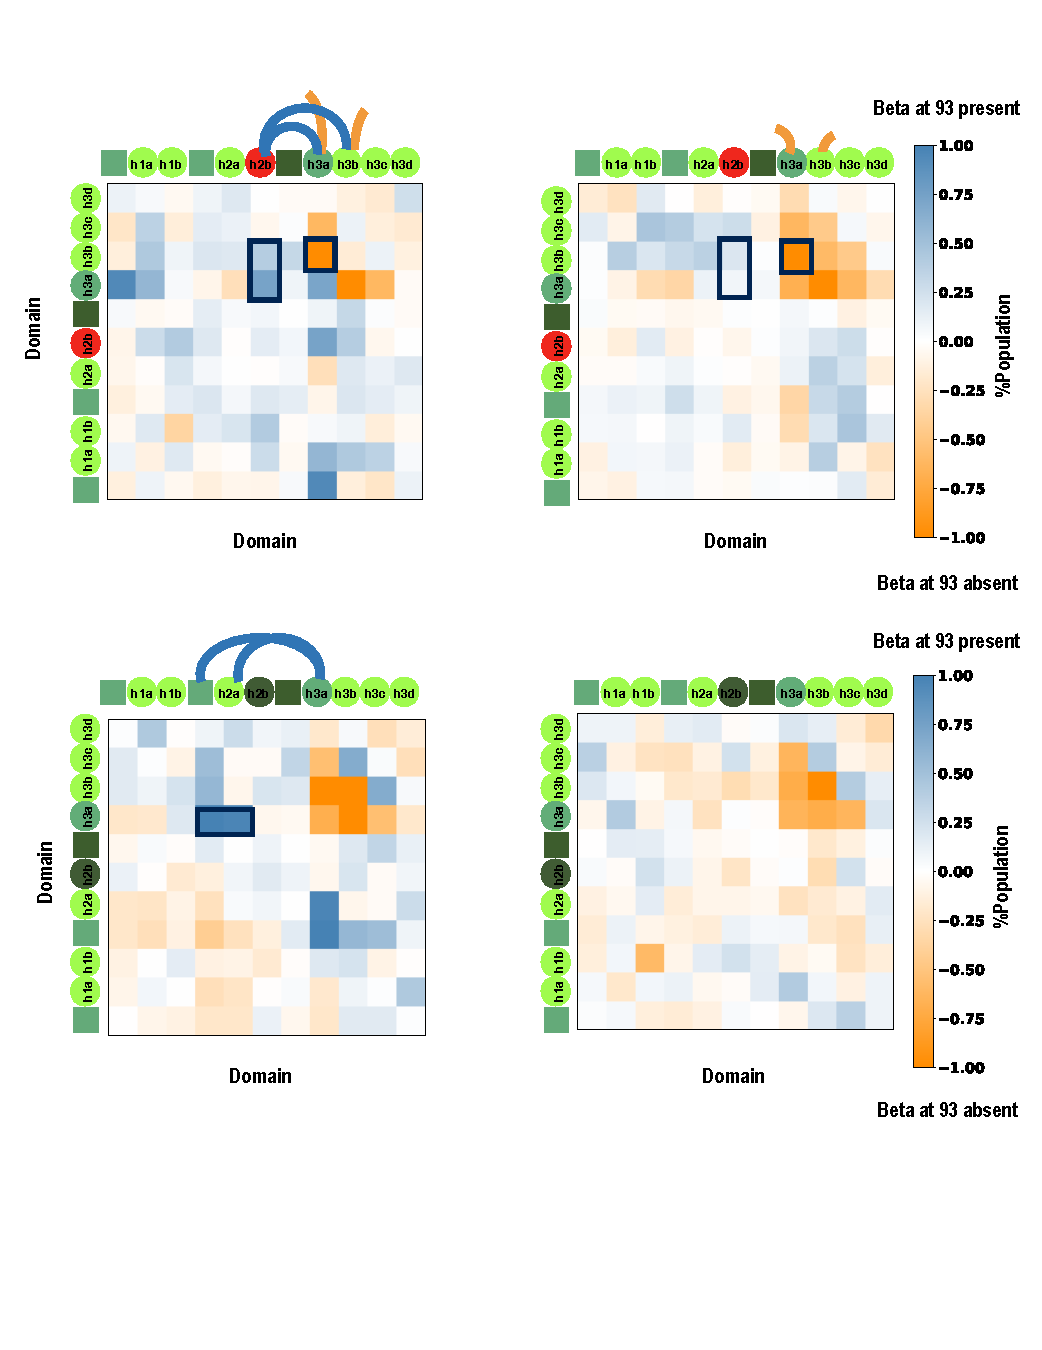
\includegraphics[scale=0.5,width=\textwidth,trim={0 0cm 0 0},clip]{../figures/S10.pdf}
\caption{{\bf Inter-domain coupling when 93 is in beta.}
.
 }
\label{S10} 
\end{figure}

\begin{figure}[!ht]
 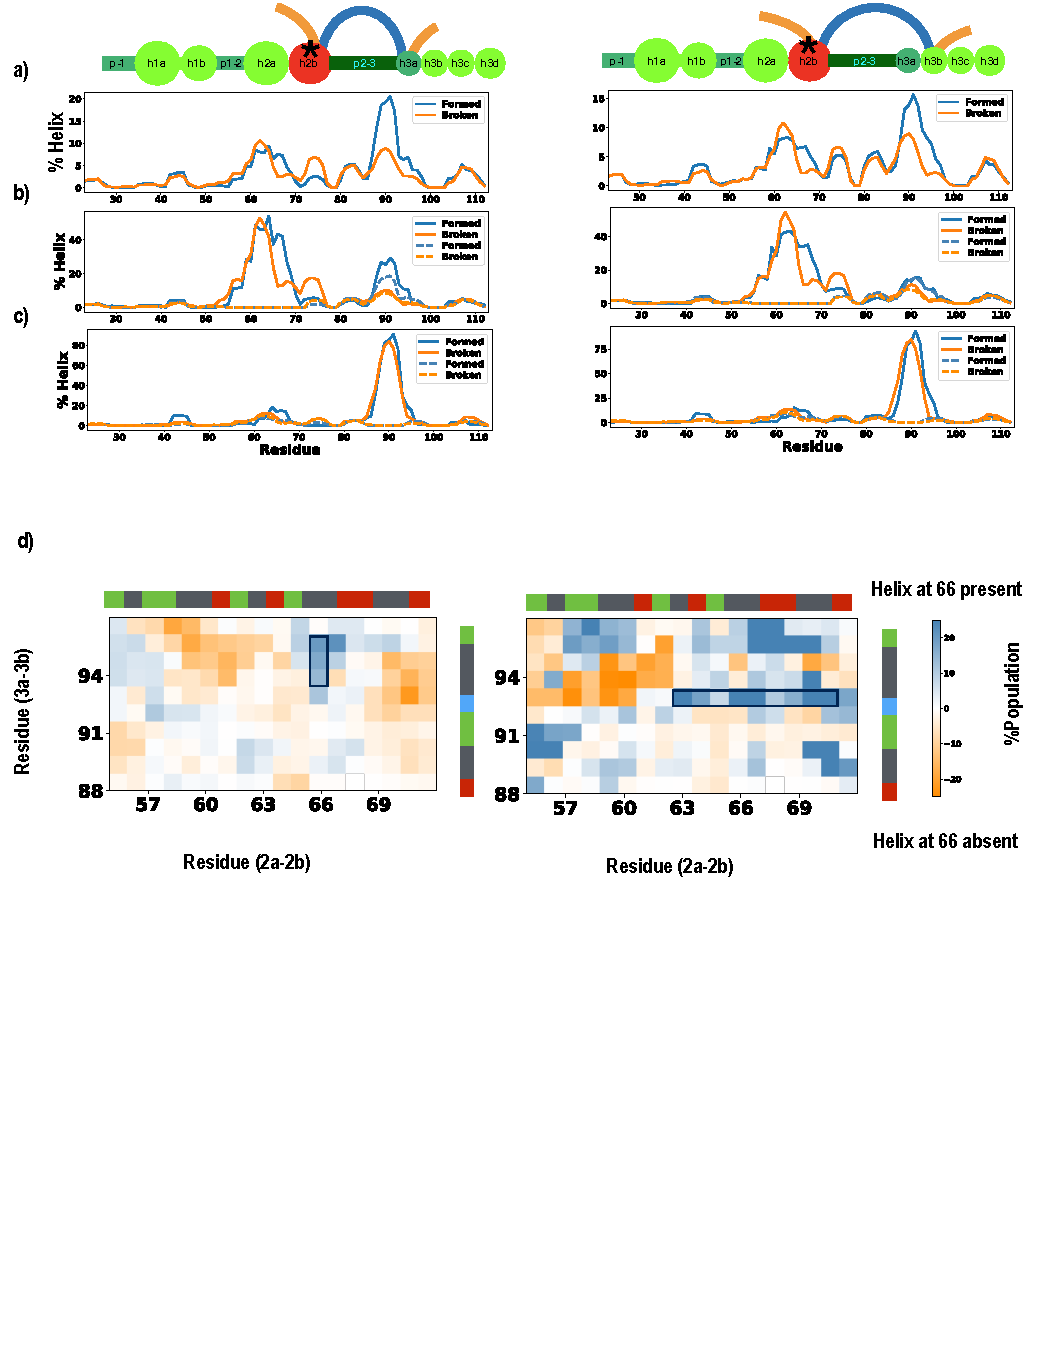
\includegraphics[scale=0.5,width=\textwidth,trim={0 0cm 0 0},clip]{../figures/S11.pdf}
\caption{{\bf Inter-domain and intra-domain coupling for M66 protonated states.}
.
 }
\label{S11} 
\end{figure}
\begin{figure}[!ht]
 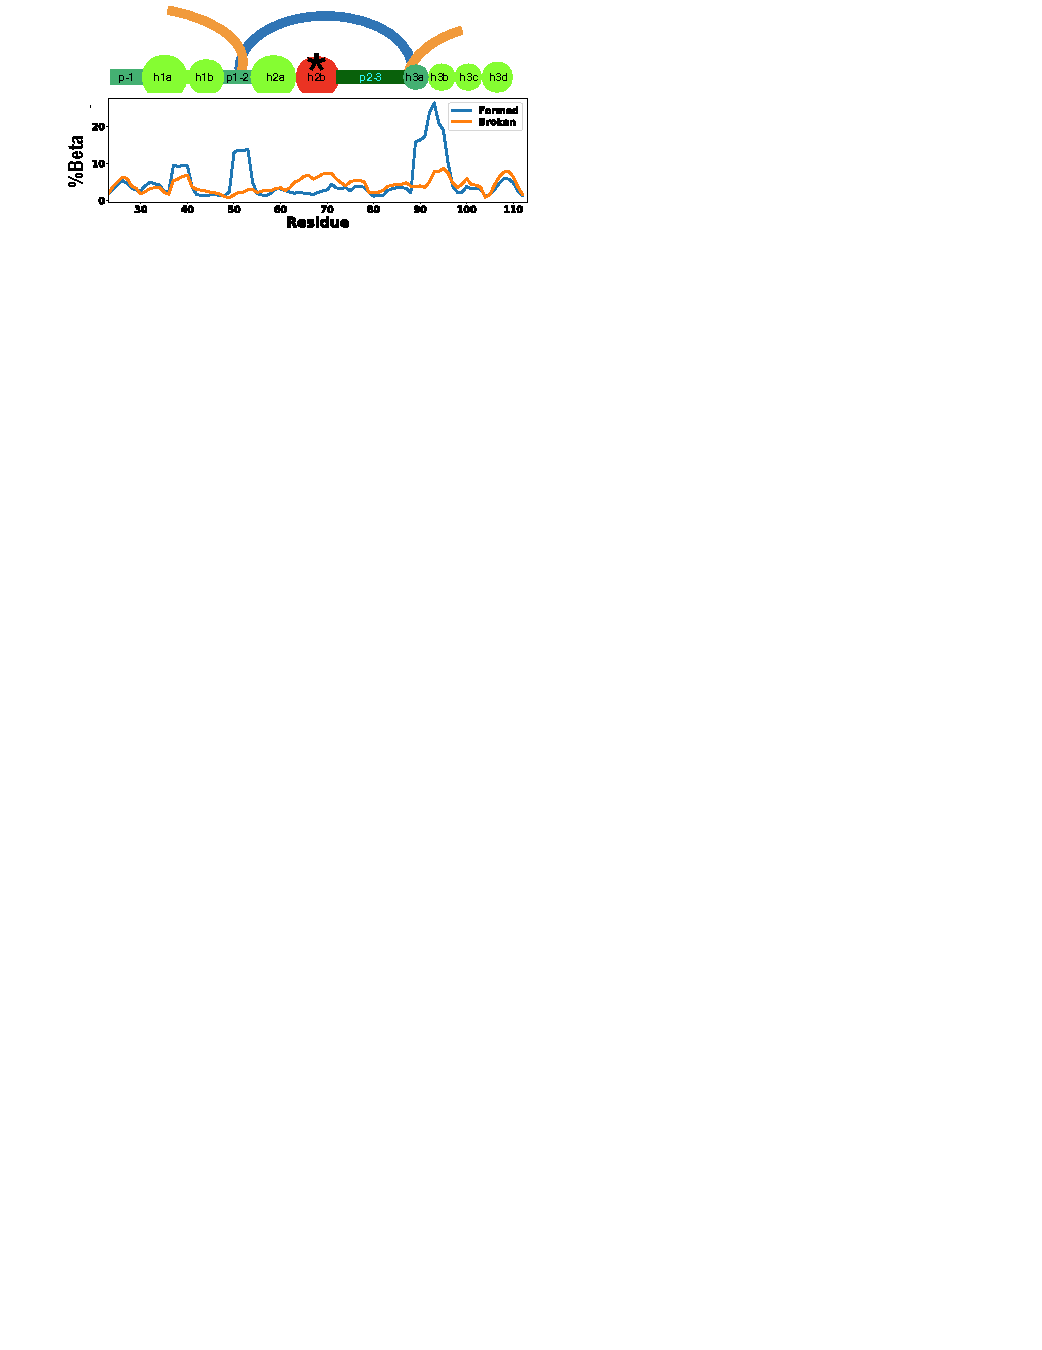
\includegraphics[scale=0.5,width=\textwidth,trim={0 0cm 0 0},clip]{../figures/S12.pdf}
\caption{{\bf Inter-domain and intra-domain coupling for V66 protonated states.}
.
 }
\label{S12} 
\end{figure}
\clearpage
\subsubsection*{Simulation convergence}
Most previous IDP simulations studies have been performed on smaller IDP fragments (residues 3-42) ~\cite{Henriques, Rauscher2017, Meng2018} . We performed the explicit solvent replica simulations of 91 residues, which was computationally challenging and thus we carefully accessed the convergence of our simulations. All replicas were able to diffuse in the temperature range 300K to 385K (replica round trip number \textgreater 7) (~\ref{S13}b). The Rg for V66 and M66 converge after 800ns of simulation at 300K (~\ref{S1}b). We discarded the first 800 ns of the trajectories as conformational equilibration.


Although there are some localized discrepancies for certain residue types (Y34,L59,M95,Y113), the discrepancy is conserved across all four simulations (FigS2). Thus, these specific discrepancies are probably reflecting residual force-field inaccuracies, including the cation-pi interactions that are poorly captured by non-polarizable force felid.

\begin{figure}[!ht]
 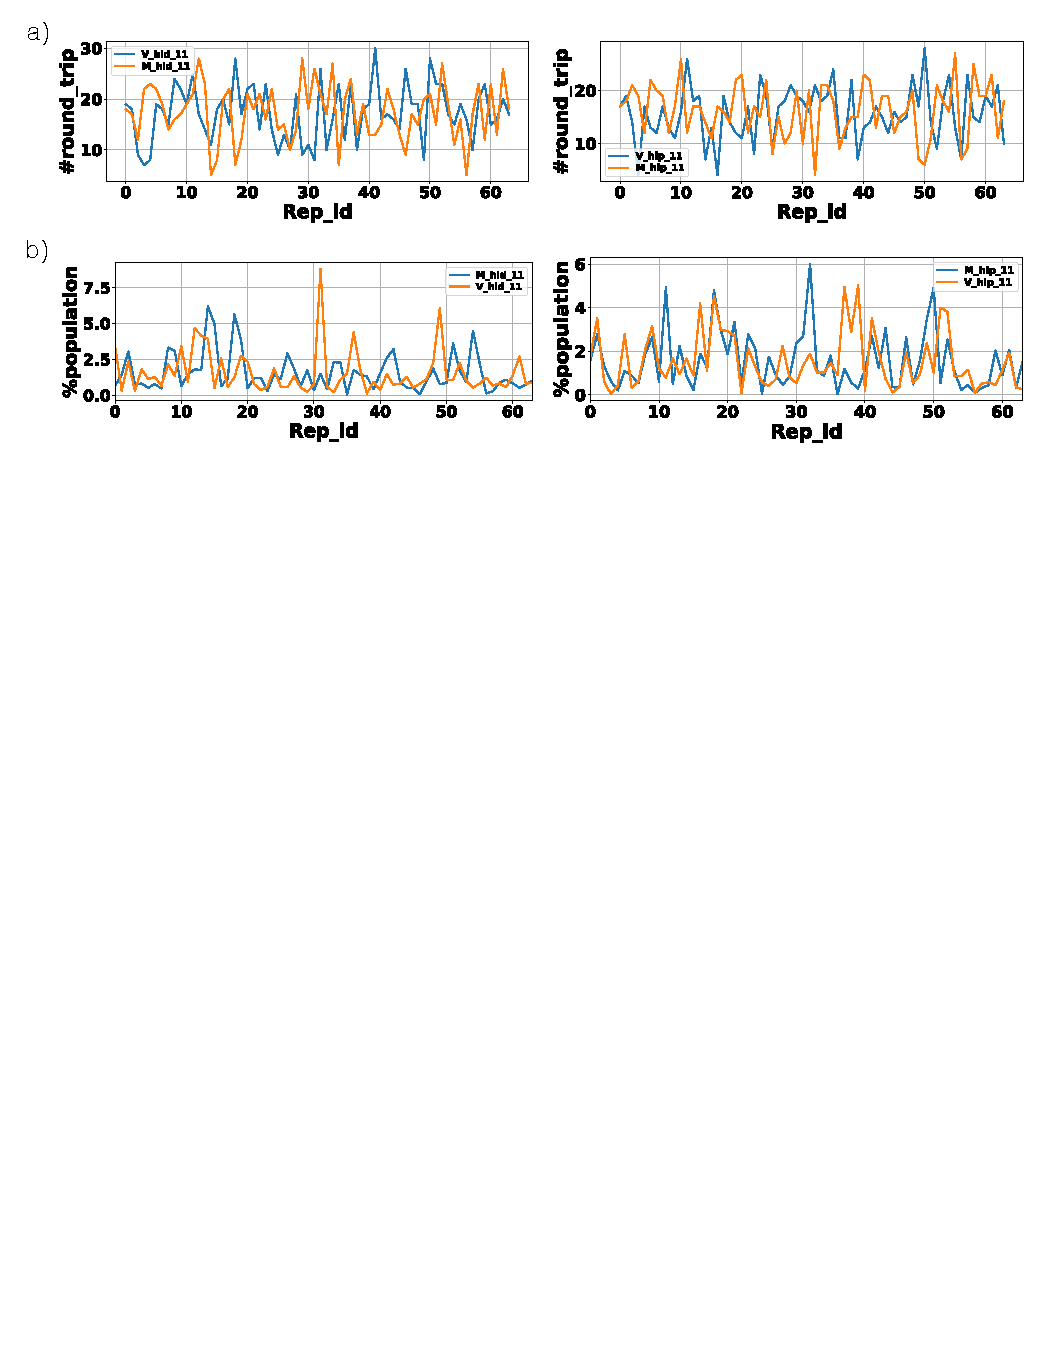
\includegraphics[scale=0.5,width=\textwidth,trim={0 0cm 0 0},clip]{../figures/S13.pdf}
\caption{{\bf Mixing of replicas during the simulation.}
Time series of blocked Rg distribution and number of round trips completed by each replica for protonated His65 and neutral His65.
 }
\label{S13} 
\end{figure}


\subsubsection*{Tertiary contacts network} The contact networks were build using Cytoscape ~\cite {Ahlstrom2013} with linear representation of residues.  Each protein residue comprises a node in the network, with interactions between residues represented as edges. The strength of individual interactions can be interpreted by the  thickness of the edge line on the network diagram. The transparency of an edge increases as it is found at more temperatures.  If residue  66 or its neighboring residues (A51-P79) are involved in h-bond formation, its edge is drawn above the node; otherwise, the edge is drawn at the bottom of the node. To focus on significant interactions, interactions showing more than 3\% persistence were considered in network visualization.      

\subsection*{Analysis of MD Trajectories} For MD simulations, the secondary structure content was  calculated with the STRIDE program incorporated in VMD,\cite{Humphrey1996}  which takes into account the combination of backbone dihedral angles and hydrogen bonding. Helix includes $\alpha$-helix and 3\textsubscript{10}-helix and $\beta$ includes $\beta$-strand and $\beta$-bridge. The hydrogen bonds were calculated with \textbar  D-A\textbar  distance \textless = .35 nm and angle D-H-A angle \textless= 40?. For salt bridges, distance \textless = .32 nm was used as cutoff between the anionic and cationic atom. The radius of gyration was calculated using the all atoms.

\subsubsection*{Hydrodynamic radius calculation} 



%\subsubsection{Finer resolution: Effect of Val66Met on *which* residues are doing the interaction}

%Several specific contacts are shown that are found in a significant number of frames for either V66 or M66, but not in the other one.   
%We observe few long-range contacts with significant differences in V66 and M66 with p  \textless  0.0001. \grace {The cross-over N is \~15 frames ?} .  We find that the differences we observe in long-range contacts are strongly correlated with contacts at residue 66,67 (i) and (i-3).
%
%Conventional contact maps provided little useful insight into tertiary structure for either forms of the protein, which was consistent with the intrinsic disorder and frequent transient interactions among neutral side-chains. Identification of contact residues yielded several persistent, weak long-range interactions at 300K for both sequences, which can be represented along a single axis (Fig~\ref{fig4}). 
%

%The prodomain has several well defined regions forming long-range tertiary contacts. \grace{We need to settle on one of two options : 1) defining the sticky domains according to hydrophobicity and showing that the tertiary contacts follow or 2) defining the domains from tertiary contacts and showing that they happen to be hydrophobic.}  All the four regions identified has high density of hydrophobic residues (Fig~\ref{fig1}c). It has been frequently observed that unfolded proteins form strong hydrophobic contacts ~\cite {Dobson1998}. Thus, it's not very surprising that the disordered prodomain has the presence of persistent hydrophobic contacts. \grace{Not sure about the previous - hydrophobicity is important for aggregation in general, within and among folded and misfolded proteins, it's just not very specific.  I'd like to change this remark but let's chat about it} Charges in the hydrophobic regions seem to determine the strength of contact formed between two hydrophobic regions.  x2 region, which is negatively charged forms contact with positively charged x3 region or neutral x1 region. Compact states of IDP's due to hydrophobic interactions have been observed in the past as well ~\cite {Chebaro2015, Kizilsavas2017}.

%\section{OLD Results and discussion}

%\newcommand{\tdomain1}{\d1}
%\newcommand{\tdomain2}{d1}



%types(Y34, Y113, R93, R27)


%\subsubsection*{Most long range contacts occur among 4 well-defined regions} 
%
%Conventional contact maps provided little useful insight into tertiary structure for either forms of the protein, which was consistent with the intrinsic disorder and frequent transient interactions among neutral side-chains. Identification of contact residues yielded several persistent, weak long-range interactions at 300K for both sequences, which can be represented along a single axis (Fig~\ref{fig4}). 
%

%Prodomain has well defined regions forming long-range tertiary contacts. All the four regions identified has high density of hydrophobic residues (Fig~\ref{fig1}c). It has been frequently observed that unfolded proteins form strong hydrophobic contacts ~\cite {Dobson1998}. Thus, it's not very surprising that the disordered prodomain has the presence of persistent hydrophobic contacts. Charges in the hydrophobic regions seem to determine the strength of contact formed between two hydrophobic regions.  x2 region, which is negatively charged forms contact with positively charged x3 region or neutral x1 region. Compact states of IDP's due to hydrophobic interactions have been observed in the past as well ~\cite {Chebaro2015, Kizilsavas2017}.


%\begin{figure}[!ht]
%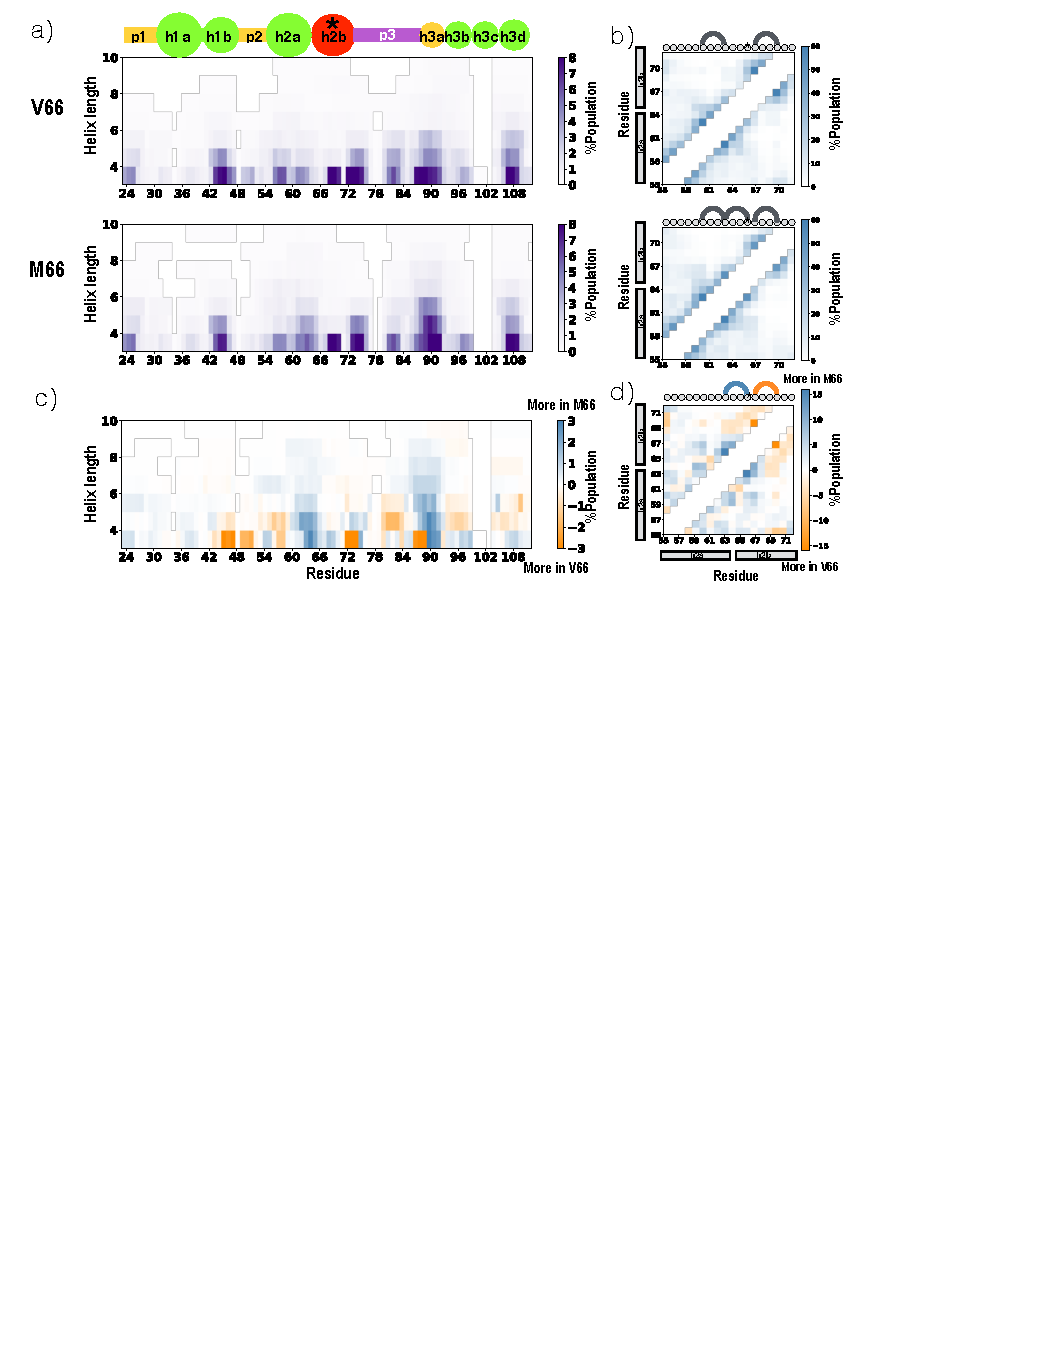
\includegraphics[scale=0.5,width=\textwidth,trim={0 0cm 0 0cm},clip]{../figures/fig5.pdf}
%
%\pagebreak
%
%\caption{{\bf Contacts formed at residue i and i-3.}
%Weight of contact formed at every residue pair separated with two residues (residue i and i-3) for V66 and M66 (top).  Difference in V66 and M66 residue pair contacts(bottom). M66 forms strong contact at residue M66:F63, whereas V66 forms strong contact at residue I67:L70.}
%
%
%\label{fig5} 
%\end{figure}
%Increased helix formation in M66 is contributed by two factors. 
%a) Reduced entropic cost of helix formation in M66 when compared with V66. Creamer et. al. ranked the entropic cost of helix formation for apolar side chains using simulations of a (Ala)\textsubscript{8} sequence with the 'guest' amino acid at the center and reported higher entropic cost helix formation for Valine when compared with Methionine \cite{Creamer1992}. 
%
%b) Helix stabilization in M66 by preferential contact formed between M66:F63. We looked at the weight of the contact formed at every residue pair separated with two residues (Fig~\ref{fig5}). Either two hydrophobic residues (L43:V46, A60:F63,A87:Y90 ) or  two residues with opposite charge (E73:K76), commonly form strong contacts (\textgreater 65\%) for both V66 and M66. Additionally, M66 forms strong contact at residue M66:F63, whereas V66 forms strong contact at residue I67:L70. A previous study from Faure et al ~\cite {Faure2008} analyzed the frequency of two amino acids contact within 1230 protein chains from Protein DataBank (PDB) and found that Methionine (M) has also a strong affinity with Phenylalanine (F) and itself.
%

%
%We also look at the temperature dependence of helical structure in prodomain. At 385K, the helix at residue 66 increases (\textgreater 2\%) for all V66, M66, V66\textsuperscript{65+}, but M66\textsuperscript{65+} has strongest preference (\textgreater 5\%) (Fig~\ref{fig4}c). Thus,  increased hydrophobic interaction with temperature (F63:M66) along with reduced electrostatic repulsion (H65:E69) in M66\textsuperscript{65+} favors helix formation.

%\newpage
%\subsubsection{How does Val66Met changes long range pairing}
%
%We observe few long-range contacts with significant differences in V66 and M66 with p  \textless  0.0001. \grace {The cross-over N is \~15 frames ?} . We find that the differences we observe in long-range contacts are strongly correlated with concats at residue 66,67 (i) and (i-3).
%
%\begin{figure}[!ht]
%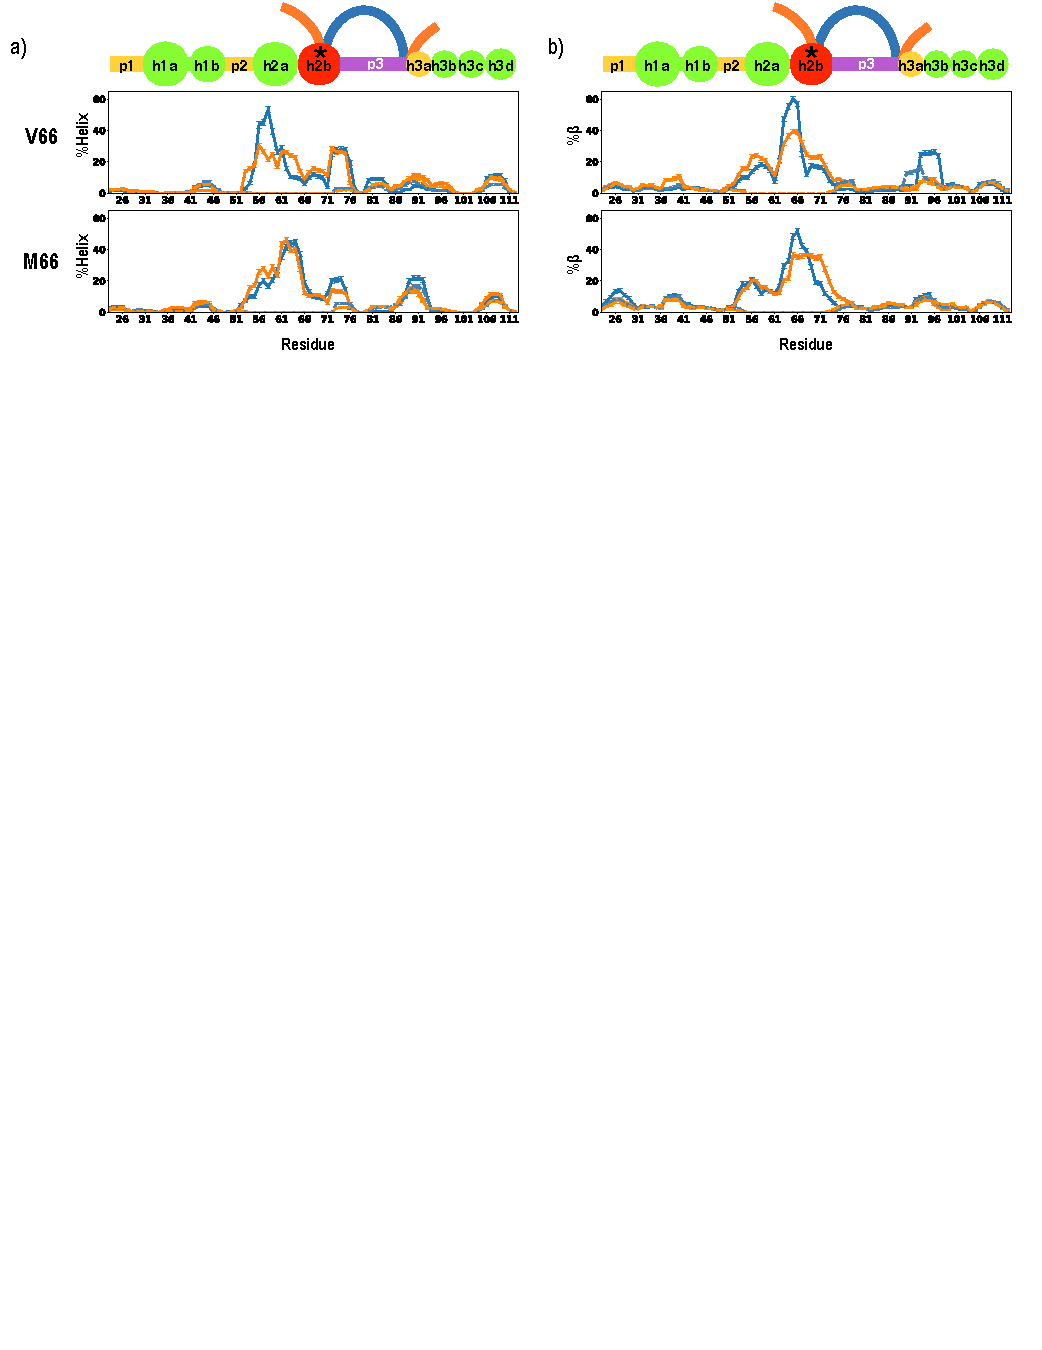
\includegraphics[scale=0.5,width=12cm,trim={0 0cm 0 0cm},clip]{../figures/fig6.pdf}
%\caption{{\bf Long range contacts are correlated with short range contact at residues 63, 65, 66 or 67, 69.} Two strongest non-correlated long range contact formed in V66 a) and M66 b). 
% }
%\label{fig6}
%\end{figure}




%\subsubsection{M66 supports helix formation at residue 93}
%
%We next examined the increased helix tendency at residue 93 from Val66Met substitution. We find structures forming helix at 93 are in contact with residue 66 in at-least 25\% of it's population in M66\textsuperscript{65+} (Fig~\ref{fig6}). The gain of this residue specific interaction in M66, probably increases helix formation at 93 when compared with V66. 
%
%\begin{figure}[!ht]
%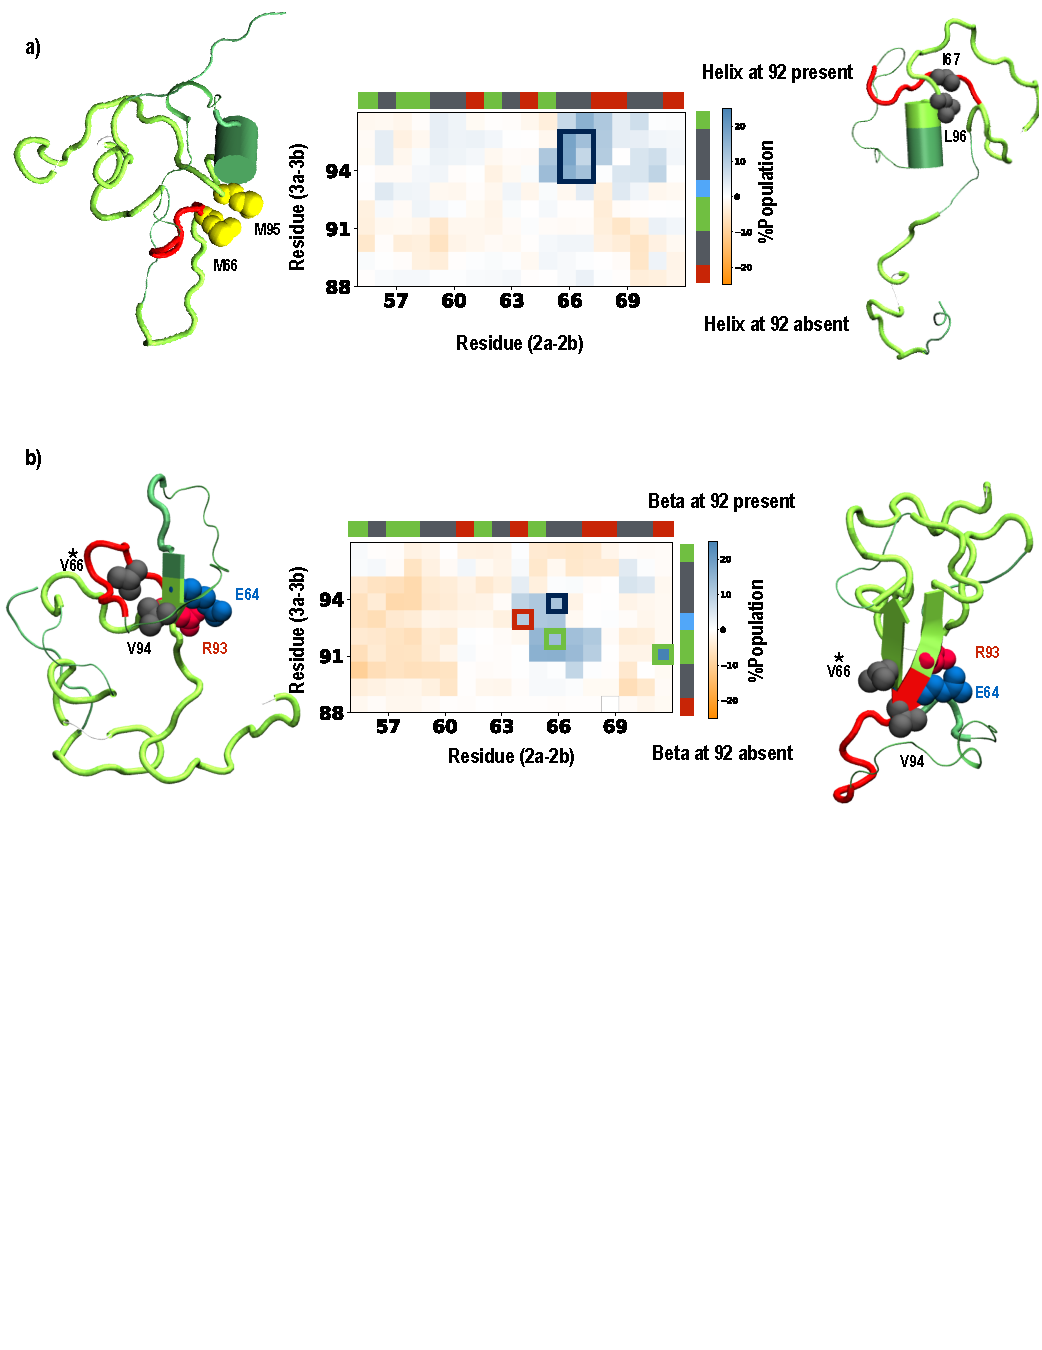
\includegraphics[scale=0.5,width=\textwidth,trim={0 0cm 0 0cm},clip]{../figures/fig8.pdf}
%
%\caption{{\bf Simulation predicted helical structure and it's comparison with experiments.} }
%
%\label{fig8} 
%\end{figure}


%\textbf{Only Val66 and not Met66 forms long beta sheet structures at residue 66 and 93.} We next examined the backbone contacts formed between residues.
%% Hip65 reduces beta sheet tendency at residue 66 for both V and M form (Fig~\ref{fig5}a). This could be due to gain of helix at 66 in Hip65 form or due to loss of sheet structures which involved salt-bridge formation at 64. 
%V66 and M66 forms differential backbone contact at residue 66 (Fig~\ref{fig5}a). V66 forms beta sheet structures with residue 92. This is also consistent with NMR observation ~\cite{Anastasia2013}  , where Val66Met changes CS at residue 93 (Fig~\ref{fig8}a) . 
%We further test if the beta sheet structures at residue 66-95 in V66 is more favored in V66 than in M66 and is not a limitation of simulation convergence. To verify this observation, we performed simulations with backbone restraints of 1Kj/mole/nm2 of a V66 frame having beta sheet structures at residue 66-95 with Val66 mutated to Met. We find that M66 has higher loss in entropy at 93 (Fig~\ref{fig5}b). Additionally, 66-92 beta structures forms 64-93 salt bridge simultaneously in V66(Fig~\ref{fig5}c). In our restrained simulations M66 has 50\% less probability of forming salt-bridge at residue 64-93 (Fig~\ref{fig5}d). This result suggests that beta at 66-95 is less favored in M66 due to higher entropic and energetic cost. 



\clearpage

\bibliography{Jacs_ref}

\end{document}

